% ============================================================
%  CodeCell C6 Drive Robot – University Presentation
%  Compile with: pdflatex → pdflatex  (two passes for overlays)
% ============================================================
\documentclass[aspectratio=169, 11pt]{beamer}

% ---------- theme & colours ----------
\usetheme{Madrid}
\usecolortheme{whale}
\setbeamertemplate{navigation symbols}{}            % hide nav buttons
\setbeamertemplate{footline}{%
  \leavevmode\hbox{%
    \begin{beamercolorbox}[wd=.35\paperwidth,ht=2.5ex,dp=1.125ex,leftskip=.3cm]{author in head/foot}%
      \usebeamerfont{author in head/foot}\insertshortauthor
    \end{beamercolorbox}%
    \begin{beamercolorbox}[wd=.40\paperwidth,ht=2.5ex,dp=1.125ex,center]{title in head/foot}%
      \usebeamerfont{title in head/foot}\insertshorttitle
    \end{beamercolorbox}%
    \begin{beamercolorbox}[wd=.25\paperwidth,ht=2.5ex,dp=1.125ex,rightskip=.3cm plus1fil]{date in head/foot}%
      \hfill\insertframenumber\,/\,\inserttotalframenumber
    \end{beamercolorbox}%
  }%
}

% ---------- packages ----------
\usepackage[T1]{fontenc}
\usepackage{lmodern}    % available on Overleaf; remove if compiling locally without texlive-fonts-extra
\usepackage{tikz}
\usetikzlibrary{
  arrows.meta, positioning, calc, shapes.geometric,
  decorations.pathreplacing, fit, backgrounds
}
\usepackage{listings}
\usepackage{booktabs}
\usepackage{amsmath}
\usepackage{graphicx}
\usepackage{xcolor}
\usepackage{textcomp}
\newcommand{\fitdiagram}[1]{\resizebox{\linewidth}{!}{#1}}

% ---------- listing style ----------
\lstset{
  basicstyle=\ttfamily\scriptsize,
  keywordstyle=\color{blue!80!black}\bfseries,
  commentstyle=\color{gray},
  stringstyle=\color{orange!80!black},
  breaklines=true,
  frame=single,
  rulecolor=\color{gray!40},
  backgroundcolor=\color{gray!5},
  numbers=none,
  showstringspaces=false,
  tabsize=2
}

% ---------- custom colours for diagrams ----------
\definecolor{hw}{HTML}{2E86C1}        % hardware blue
\definecolor{sw}{HTML}{27AE60}        % software green
\definecolor{comm}{HTML}{E67E22}      % communication orange
\definecolor{ctrl}{HTML}{8E44AD}      % control purple
\definecolor{danger}{HTML}{C0392B}    % safety red
\definecolor{lightbg}{HTML}{EBF5FB}   % light background

% ---------- meta ----------
\title[CodeCell C6 Drive Robot]{Differential-Drive Robot\\with the CodeCell C6 Drive}
\subtitle{Design, Control \& Wireless Operation}
\author[K. Sawicki, M. Szerechowicz, M. Skorupiński]{Krzysztof Sawicki, Michał Szerechowicz, Mateusz Skorupiński}
\institute[]{Poznań University of Technology \\ Automation Control and Robotics\\[6pt]
Supervisor: Dr. Eng. Marek Kraft}
\date{\today}

\setbeameroption{show notes on second screen=right}

% ============================================================
\begin{document}

% ---- TITLE ----
\begin{frame}[plain]
  \titlepage
\end{frame}
\note{
Introduce the project as a compact differential-drive robot built around the CodeCell C6 Drive board. Mention that the presentation covers the mechanical layout, electronics, control software, wireless interface, and safety mechanisms.
}

% ---- OUTLINE ----
\begin{frame}{Outline}
  \tableofcontents
\end{frame}
\note{
Briefly walk through the structure: project goals, hardware, mechanical design, software architecture, movement control, wireless communication, browser interface, safety, and future work. Keep this slide short and use it only as orientation.
}

% ============================================================
\section{Project Overview}
% ============================================================

\begin{frame}{Project Goals}

  \begin{columns}[T]
    \begin{column}{0.55\textwidth}
      Build a \textbf{compact, wirelessly controlled} differential-drive robot
      using the CodeCell~C6~Drive as the sole electronic module.

      \bigskip
      \textbf{Key objectives:}
      \begin{itemize}
        \item Heading-stabilised motion via onboard IMU
        \item Two operating modes: real-time joystick \&
              autonomous point-to-point
        \item Browser-based control app (no install needed)
        \item 3D-printed chassis – reproducible build
      \end{itemize}
    \end{column}

    \begin{column}{0.42\textwidth}
      \centering
      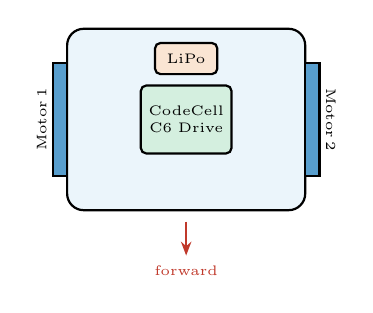
\begin{tikzpicture}[scale=0.72, every node/.style={font=\small}]
        % Chassis body
        \fill[lightbg, rounded corners=6pt]
          (-2.1,-1.6) rectangle (2.1,1.6);
        \draw[thick, rounded corners=6pt]
          (-2.1,-1.6) rectangle (2.1,1.6);

        % Left wheel
        \fill[hw!80] (-2.35,-1.0) rectangle (-2.1,1.0);
        \draw[thick] (-2.35,-1.0) rectangle (-2.1,1.0);
        \node[font=\tiny, rotate=90] at (-2.55,0) {Motor\,1};

        % Right wheel
        \fill[hw!80] (2.1,-1.0) rectangle (2.35,1.0);
        \draw[thick] (2.1,-1.0) rectangle (2.35,1.0);
        \node[font=\tiny, rotate=-90] at (2.55,0) {Motor\,2};

        % Board
        \fill[sw!20, rounded corners=2pt]
          (-0.8,-0.6) rectangle (0.8,0.6);
        \draw[thick, rounded corners=2pt]
          (-0.8,-0.6) rectangle (0.8,0.6);
        \node[font=\tiny, text width=1.4cm, align=center] at (0,0)
          {CodeCell\\C6 Drive};

        % Battery
        \fill[comm!20, rounded corners=2pt]
          (-0.55,0.8) rectangle (0.55,1.35);
        \draw[thick, rounded corners=2pt]
          (-0.55,0.8) rectangle (0.55,1.35);
        \node[font=\tiny] at (0,1.07) {LiPo};

        % Forward arrow
        \draw[-{Stealth[length=5pt]}, thick, danger]
          (0,-1.8) -- (0,-2.4) node[below, font=\tiny]{forward};

      \end{tikzpicture}

      \smallskip
      {\scriptsize Top-down schematic view}
    \end{column}
  \end{columns}
\end{frame}
\note{
Explain that the main idea was to build a small mobile robot with minimal external electronics. Emphasize that the CodeCell C6 Drive acts as the core module: motor driver, wireless interface, and sensor platform. Point out the two modes: direct joystick control and autonomous target movement.
}

% ============================================================
\section{Hardware}
% ============================================================

\begin{frame}{CodeCell C6 Drive – Board Overview}

  \centering
  \fitdiagram{%
  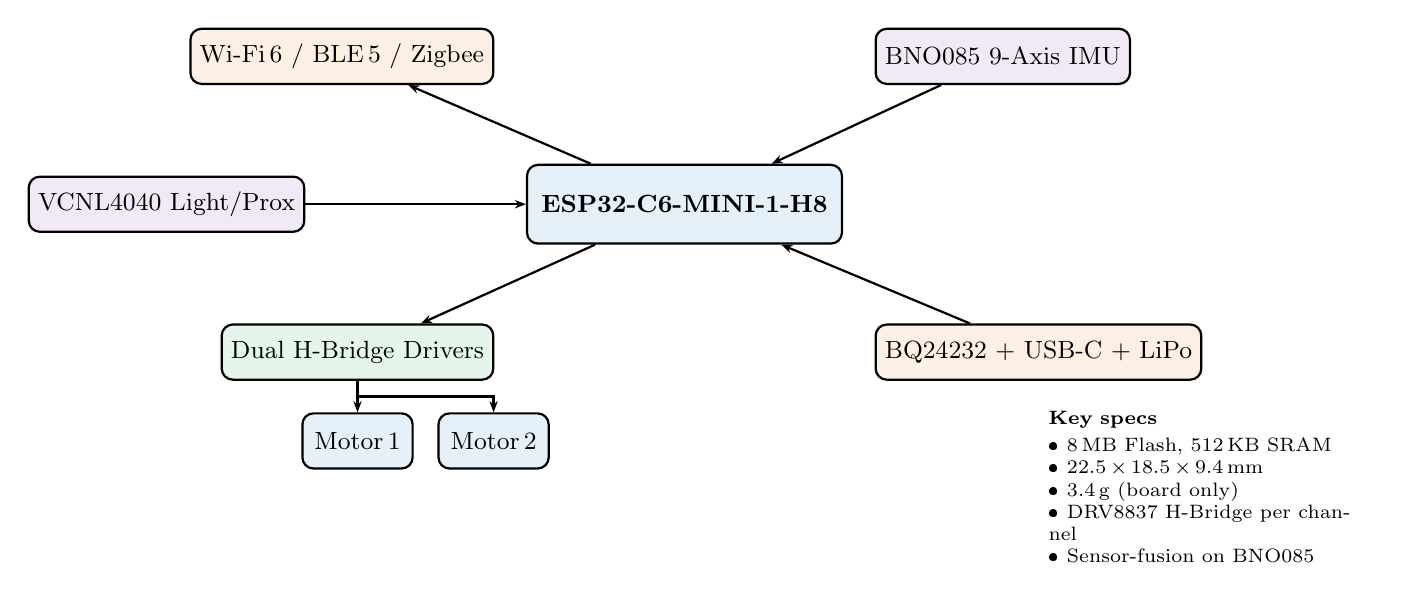
\begin{tikzpicture}[
      every node/.style={font=\small},
      box/.style={draw, thick, rounded corners=4pt,
                  minimum width=3.2cm, minimum height=0.7cm,
                  text=black},
      arr/.style={-{Stealth[length=4pt]}, thick}
    ]
    % Central MCU
    \node[box, fill=hw!12, minimum width=4cm, minimum height=1cm]
      (mcu) {\textbf{ESP32-C6-MINI-1-H8}};

    % Peripherals
    \node[box, fill=comm!12, above left=1cm and 0.4cm of mcu] (wifi)
      {Wi-Fi\,6 / BLE\,5 / Zigbee};
    \node[box, fill=ctrl!12, above right=1cm and 0.4cm of mcu] (imu)
      {BNO085 9-Axis IMU};
    \node[box, fill=sw!12, below left=1cm and 0.4cm of mcu]  (drv)
      {Dual H-Bridge Drivers};
    \node[box, fill=comm!12, below right=1cm and 0.4cm of mcu] (pwr)
      {BQ24232 + USB-C + LiPo};
    \node[box, fill=ctrl!12, left=2.8cm of mcu] (prox)
      {VCNL4040 Light/Prox};

    \draw[arr] (mcu) -- (wifi);
    \draw[arr] (imu) -- (mcu);
    \draw[arr] (mcu) -- (drv);
    \draw[arr] (pwr) -- (mcu);
    \draw[arr] (prox) -- (mcu);

    % Motors
    \node[box, fill=hw!12, below=0.4cm of drv, minimum width=1.4cm]
      (m1) {Motor\,1};
    \node[box, fill=hw!12, right=0.3cm of m1, minimum width=1.4cm]
      (m2) {Motor\,2};
    \draw[arr] (drv.south) -- ++(0,-0.2) -| (m1.north);
    \draw[arr] (drv.south) -- ++(0,-0.2) -| (m2.north);

    % Specs
    \node[anchor=north west, font=\scriptsize, text width=4cm,
          align=left] at (4.5,-2.5) {%
      \textbf{Key specs}\\[2pt]
      \textbullet~8\,MB Flash, 512\,KB SRAM\\
      \textbullet~22.5\,$\times$\,18.5\,$\times$\,9.4\,mm\\
      \textbullet~3.4\,g (board only)\\
      \textbullet~DRV8837 H-Bridge per channel\\
      \textbullet~Sensor-fusion on BNO085
    };
  \end{tikzpicture}
  }
\end{frame}
\note{
Describe the board as the central hardware element. Highlight the ESP32-C6 for computation and wireless communication, the BNO085 IMU for heading estimation, the motor drivers for the two wheels, and the LiPo/USB-C power path. Mention that using one compact board simplifies wiring and makes the robot easier to reproduce.
}

% ============================================================

\begin{frame}{Mechanical Design}

  \begin{columns}[T]
    \begin{column}{0.45\textwidth}
      \textbf{Differential-drive layout}
      \begin{itemize}
        \item Left motor $\rightarrow$ left wheel
        \item Right motor $\rightarrow$ right wheel
        \item Board and LiPo mounted centrally
      \end{itemize}

      \bigskip
      \textbf{Chassis}
      \begin{itemize}
        \item 3D-printed (FDM), single-piece shell
        \item Designed for press-fit motor mounting
      \end{itemize}

      \bigskip
      \textbf{Turning principle}\\[4pt]
      {\small
        Equal speed $\Rightarrow$ straight line\\
        Speed difference $\Rightarrow$ curved path\\
        Opposite speeds $\Rightarrow$ rotation in place
      }
    \end{column}

    \begin{column}{0.52\textwidth}
      \centering
      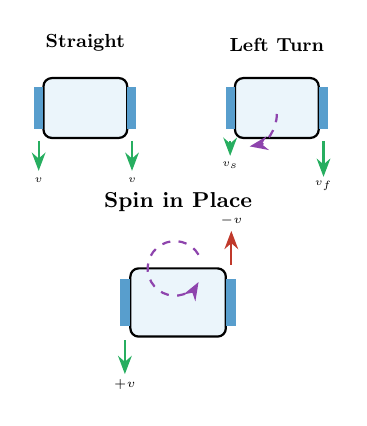
\begin{tikzpicture}[scale=0.76, every node/.style={font=\small}, transform shape]
        % --- straight ---
        \begin{scope}[shift={(-1.55,2.1)}]
          \fill[lightbg, rounded corners=3pt] (-0.7,-0.5) rectangle (0.7,0.5);
          \draw[thick, rounded corners=3pt] (-0.7,-0.5) rectangle (0.7,0.5);
          \fill[hw!80] (-0.85,-0.35) rectangle (-0.7,0.35);
          \fill[hw!80] (0.7,-0.35) rectangle (0.85,0.35);
          \draw[-{Stealth},thick,sw] (-0.78,-0.55) -- (-0.78,-1.05);
          \draw[-{Stealth},thick,sw] ( 0.78,-0.55) -- ( 0.78,-1.05);
          \node[font=\tiny] at (-0.78,-1.2) {$v$};
          \node[font=\tiny] at ( 0.78,-1.2) {$v$};
          \node[above, font=\small\bfseries] at (0,0.82) {Straight};
        \end{scope}
        % --- left turn ---
        \begin{scope}[shift={(1.65,2.1)}]
          \fill[lightbg, rounded corners=3pt] (-0.7,-0.5) rectangle (0.7,0.5);
          \draw[thick, rounded corners=3pt] (-0.7,-0.5) rectangle (0.7,0.5);
          \fill[hw!80] (-0.85,-0.35) rectangle (-0.7,0.35);
          \fill[hw!80] (0.7,-0.35) rectangle (0.85,0.35);
          \draw[-{Stealth},thick,sw] (-0.78,-0.55) -- (-0.78,-0.80);
          \draw[-{Stealth},thick,sw] ( 0.78,-0.55) -- ( 0.78,-1.15);
          \node[font=\tiny] at (-0.78,-0.95) {$v_s$};
          \node[font=\tiny] at ( 0.78,-1.3) {$v_f$};
          \node[above, font=\small\bfseries] at (0,0.82) {Left Turn};
          \draw[-{Stealth},thick,ctrl,dashed] (0,-0.1)
            arc[start angle=0,end angle=-80,radius=0.55];
        \end{scope}
        % --- spin ---
        \begin{scope}[shift={(0,-1.15)}, scale=1.14]
          \fill[lightbg, rounded corners=3pt] (-0.7,-0.5) rectangle (0.7,0.5);
          \draw[thick, rounded corners=3pt] (-0.7,-0.5) rectangle (0.7,0.5);
          \fill[hw!80] (-0.85,-0.35) rectangle (-0.7,0.35);
          \fill[hw!80] (0.7,-0.35) rectangle (0.85,0.35);
          \draw[-{Stealth},thick,sw] (-0.78,-0.55) -- (-0.78,-1.05);
          \draw[-{Stealth},thick,danger] ( 0.78, 0.55) -- ( 0.78, 1.05);
          \node[font=\tiny] at (-0.78,-1.2) {$+v$};
          \node[font=\tiny] at ( 0.78, 1.2) {$-v$};
          \node[above, font=\small\bfseries] at (0,1.2) {Spin in Place};
          \draw[-{Stealth},thick,ctrl,dashed]
            (0.3,0.7) arc[start angle=30,end angle=330,radius=0.4];
        \end{scope}
      \end{tikzpicture}
    \end{column}
  \end{columns}
\end{frame}
\note{
Explain the differential-drive principle: two independently driven wheels create straight motion, turns, and rotation in place. Mention that the chassis is 3D printed and designed to hold the board, battery, and motors compactly. Use the three diagrams to show equal speed, unequal speed, and opposite wheel directions.
}

% ============================================================
\section{Software Architecture}
% ============================================================

\begin{frame}{FreeRTOS Task Architecture}

  \centering
  \fitdiagram{%
  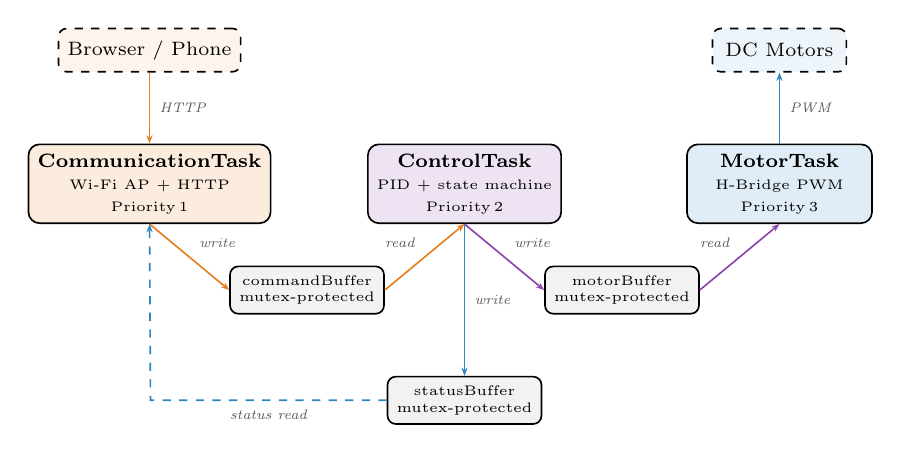
\begin{tikzpicture}[
      every node/.style={font=\scriptsize},
      task/.style={draw, semithick, rounded corners=4pt,
                   minimum width=2.35cm, minimum height=0.72cm,
                   align=center},
      buf/.style={draw, semithick, fill=gray!10, rounded corners=3pt,
                  minimum width=1.85cm, minimum height=0.46cm,
                  font=\tiny, align=center},
      arr/.style={-{Stealth[length=3pt]}, semithick},
      label/.style={font=\tiny\itshape, text=gray!70!black}
    ]

    % Tasks
    \node[task, fill=comm!15] (web) at (0,0)
      {\textbf{CommunicationTask}\\{\tiny Wi-Fi AP + HTTP}\\{\tiny Priority\,1}};
    \node[task, fill=ctrl!15] (ctl) at (4.0,0)
      {\textbf{ControlTask}\\{\tiny PID + state machine}\\{\tiny Priority\,2}};
    \node[task, fill=hw!15] (mot) at (8.0,0)
      {\textbf{MotorTask}\\{\tiny H-Bridge PWM}\\{\tiny Priority\,3}};

    % Shared buffers
    \node[buf] (cmd) at (2.0,-1.35) {commandBuffer\\{\tiny mutex-protected}};
    \node[buf] (mbuf) at (6.0,-1.35) {motorBuffer\\{\tiny mutex-protected}};
    \node[buf] (stat) at (4.0,-2.75) {statusBuffer\\{\tiny mutex-protected}};

    % Arrows
    \draw[arr, comm]  (web.south) -- node[above right, label]{write} (cmd.west);
    \draw[arr, comm]  (cmd.east) -- node[above left, label]{read} (ctl.south);
    \draw[arr, ctrl]  (ctl.south) -- node[above right, label]{write} (mbuf.west);
    \draw[arr, ctrl]  (mbuf.east) -- node[above left, label]{read} (mot.south);
    \draw[arr, hw]    (ctl.south) -- node[right, label]{write} (stat.north);
    \draw[arr, hw, dashed] (stat.west) -- ++(-3,0)
      node[midway, below, label]{status read} -- (web.south);

    % External
    \node[draw, dashed, semithick, rounded corners=3pt,
          fill=comm!8, minimum width=1.7cm, minimum height=0.55cm,
          above=0.9cm of web, font=\scriptsize]
      (browser) {Browser / Phone};
    \draw[arr, comm] (browser) -- node[right, label]{HTTP} (web);

    \node[draw, dashed, semithick, rounded corners=3pt,
          fill=hw!8, minimum width=1.7cm, minimum height=0.55cm,
          above=0.9cm of mot, font=\scriptsize]
      (motors) {DC Motors};
    \draw[arr, hw] (mot) -- node[right, label]{PWM} (motors);

  \end{tikzpicture}
  }

\end{frame}
\note{
Explain that the firmware is split into three FreeRTOS tasks. The communication task handles HTTP commands, the control task interprets commands and computes motor targets, and the motor task drives the H-bridges. Point out that shared buffers are protected by mutexes so tasks do not write over each other.
}

% ============================================================
\section{Movement Control}
% ============================================================

\begin{frame}{Differential-Drive Motor Mixing}

  \begin{columns}[T]
    \begin{column}{0.45\textwidth}
      Joystick inputs in $[-100,\,100]$:
      \begin{itemize}
        \item \texttt{move}: forward/backward
        \item \texttt{rotation}: turning
      \end{itemize}

      \smallskip
      \textbf{Mixing equations}

      \vspace{-0.35em}
      \[
      \begin{aligned}
        m_1 &= \operatorname{clip}(\texttt{move}+\texttt{rot})\\
        m_2 &= \operatorname{clip}(\texttt{move}-\texttt{rot})
      \end{aligned}
      \]
      \vspace{-0.55em}
      {\small where \(\operatorname{clip}(x)\in[-100,100]\).}
        \medskip
      {\small Sign sets direction; magnitude sets PWM duty cycle.}
    \end{column}

    \begin{column}{0.52\textwidth}
      \centering
      \resizebox{0.75\linewidth}{!}{%
      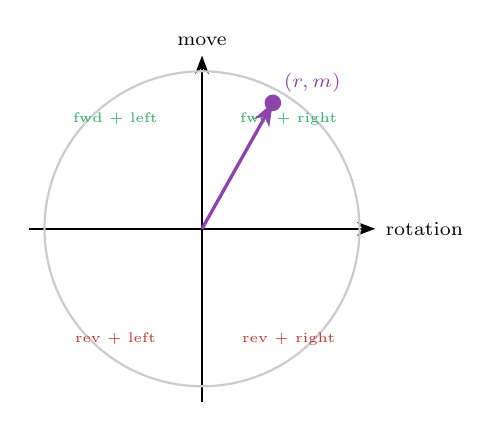
\begin{tikzpicture}[every node/.style={font=\small}]
        % Joystick axes
        \draw[-{Stealth}, thick] (-2.2,0) -- (2.2,0)
          node[right, font=\scriptsize]{rotation};
        \draw[-{Stealth}, thick] (0,-2.2) -- (0,2.2)
          node[above, font=\scriptsize]{move};
        \draw[thick, gray!40] (0,0) circle(2);

        % Quadrant labels
        \node[font=\tiny, text=sw] at ( 1.1, 1.4) {fwd + right};
        \node[font=\tiny, text=sw] at (-1.1, 1.4) {fwd + left};
        \node[font=\tiny, text=danger] at ( 1.1,-1.4) {rev + right};
        \node[font=\tiny, text=danger] at (-1.1,-1.4) {rev + left};

        % Example vector
        \draw[-{Stealth}, very thick, ctrl]
          (0,0) -- (0.9,1.6) node[above right, font=\scriptsize]{$(r, m)$};
        \fill[ctrl] (0.9,1.6) circle(3pt);

      \end{tikzpicture}
      }

      \vspace{0.05em}
      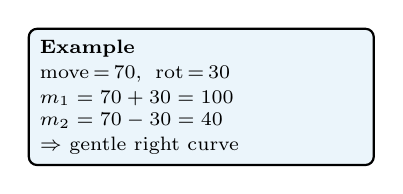
\begin{tikzpicture}
        \node[draw, thick, fill=lightbg, rounded corners=3pt,
              text width=4.1cm, align=left, font=\scriptsize,
              inner sep=4pt] {%
          \textbf{Example}\\[1pt]
          move\,=\,70,\; rot\,=\,30\\[1pt]
          $m_1 = 70+30 = 100$\\
          $m_2 = 70-30 = 40$\\[1pt]
          $\Rightarrow$ gentle right curve
        };
      \end{tikzpicture}
    \end{column}
  \end{columns}

\end{frame}
\note{
Describe how joystick input is converted into left and right motor commands. The forward/backward value is combined with the rotation value. A positive rotation increases one motor and decreases the other, creating a turn. The example shows a forward-right curve where one wheel moves faster than the other.
}

% ============================================================

\begin{frame}{Heading-Stabilised Control – PID on Yaw}

  The BNO085 provides fused \textbf{yaw} (heading) at each control cycle
  ($\sim$50\,Hz). A discrete PID controller minimises heading error and feeds
  its output as the \texttt{rotation} input to the motor mixer.

  \bigskip
  \textbf{Tuning parameters}

  \medskip
  \begin{center}
      {\small
      \begin{tabular}{@{}ll@{}}
        \toprule
        Parameter & Value \\
        \midrule
        $K_p$              & 0.30 \\
        $K_i$              & 0.02 \\
        $K_d$              & 0.02 \\
        Integral limit     & $\pm$\,120 \\
        Max correction     & $\pm$\,45 \\
        \bottomrule
      \end{tabular}
      }
  \end{center}

  \bigskip
  Error is wrapped to $(-180^\circ,\,180^\circ]$ so the controller always uses
  the shortest rotation path.
\end{frame}
\note{
Explain that the BNO085 gives a fused yaw angle, which is more useful than raw accelerometer or gyro data alone. The controller compares the desired heading with the measured heading. The PID constants were chosen conservatively so the robot corrects drift without oscillating strongly.
}

\begin{frame}{PID Yaw Feedback Loop}
  \centering
  \resizebox{0.92\linewidth}{!}{%
      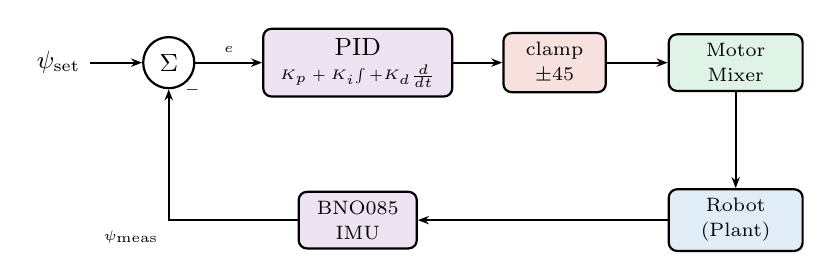
\begin{tikzpicture}[
          every node/.style={font=\small},
          block/.style={draw, thick, rounded corners=3pt,
                        minimum width=1.6cm, minimum height=0.7cm,
                        align=center},
          sum/.style={draw, thick, circle, minimum size=0.5cm, fill=white},
          arr/.style={-{Stealth[length=4pt]}, thick}
        ]

        % Setpoint
        \node (sp) at (-3.8,0) {$\psi_{\text{set}}$};

        % Summing junction
        \node[sum] (s) at (-2.4,0) {\small$\Sigma$};

        % PID
        \node[block, fill=ctrl!15, minimum width=2.4cm] (pid) at (0,0) {PID\\[-2pt]{\tiny$K_p + K_i\!\int + K_d\frac{d}{dt}$}};

        % Clamp
        \node[block, fill=danger!15, minimum width=1.3cm] (clamp) at (2.5,0)
          {\scriptsize clamp\\[-2pt]\scriptsize$\pm 45$};

        % Mixer
        \node[block, fill=sw!15, minimum width=1.7cm] (mix) at (4.8,0)
          {\scriptsize Motor\\[-2pt]\scriptsize Mixer};

        % Plant
        \node[block, fill=hw!15, minimum width=1.7cm] (plant) at (4.8,-2.0)
          {\scriptsize Robot\\[-2pt]\scriptsize (Plant)};

        % IMU
        \node[block, fill=ctrl!15, minimum width=1.5cm] (imu) at (0,-2.0)
          {\scriptsize BNO085\\[-2pt]\scriptsize IMU};

        % Arrows
        \draw[arr] (sp)    -- (s);
        \draw[arr] (s)     -- node[above,font=\tiny]{$e$} (pid);
        \draw[arr] (pid)   -- (clamp);
        \draw[arr] (clamp) -- (mix);
        \draw[arr] (mix)   -- (plant);
        \draw[arr] (plant) -- (imu);
        \draw[arr] (imu)   -| node[below left,font=\tiny]{$\psi_{\text{meas}}$} (s);

        % Negative sign
        \node[font=\tiny] at (-2.1,-0.35) {$-$};
      \end{tikzpicture}
  }
\end{frame}
\note{
Walk through the feedback loop from left to right. The set heading is compared with measured heading, PID produces a correction, the correction is clamped, and the motor mixer applies it to the wheels. The robot motion changes the measured yaw, closing the loop through the IMU.
}

% ============================================================

\begin{frame}{Control Modes – Direct vs.\ Target}

  \centering
  {\small Both modes are selected by the REST API command sent to the robot.}

  \bigskip
  \begin{columns}[T]
    \begin{column}{0.47\textwidth}
      \setbeamercolor{block title}{fg=white,bg=sw!80}
      \setbeamercolor{block body}{bg=sw!8}
      \begin{block}{\centering Direct Mode (Joystick)}
        \begin{itemize}
          \item Joystick sends (\texttt{move}, \texttt{rotation})
                at 10\,Hz via HTTP
          \item \texttt{rotation} $\rightarrow$ yaw rate
                (degrees/s scaling)
          \item PID maintains heading setpoint
          \item Stick release $\rightarrow$ auto-centre,
                sends (0,\,0) $\rightarrow$ stop
        \end{itemize}
      \end{block}
    \end{column}

    \begin{column}{0.47\textwidth}
      \setbeamercolor{block title}{fg=white,bg=ctrl!80}
      \setbeamercolor{block body}{bg=ctrl!8}
      \begin{block}{\centering Target Mode (Autonomous)}
        \begin{itemize}
          \item User specifies distance\,(m)
                and angle\,($^\circ$)
          \item Phase\,1: rotate to target heading
          \item Phase\,2: drive straight with
                PID yaw correction
          \item Distance by timer \emph{or} IMU
        \end{itemize}
      \end{block}
    \end{column}
  \end{columns}
\end{frame}
\note{
Compare the two control modes. Direct mode is for manual driving from the browser joystick and continuously sends movement commands. Target mode is more autonomous: the user gives a distance and angle, and the robot executes the motion in phases.
}

% ============================================================

\begin{frame}{Target Mode – Two-Phase Execution}

  \centering
  \fitdiagram{%
  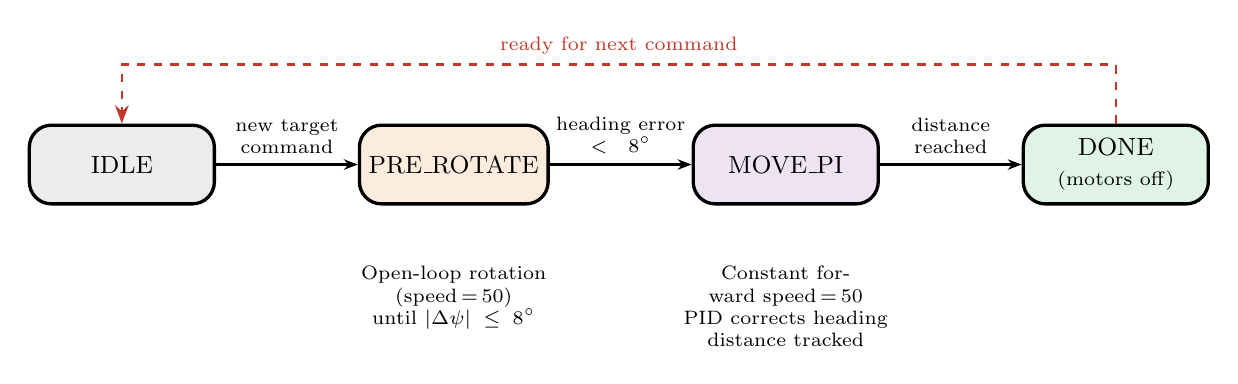
\begin{tikzpicture}[
      every node/.style={font=\small},
      state/.style={draw, very thick, rounded corners=8pt,
                    minimum width=2.35cm, minimum height=1.0cm,
                    align=center},
      arr/.style={-{Stealth[length=5pt]}, very thick},
      note/.style={font=\scriptsize, text width=2.7cm, align=center}
    ]

    \node[state, fill=gray!15] (idle) {IDLE};
    \node[state, fill=comm!15, right=1.8cm of idle] (pre) {PRE\_ROTATE};
    \node[state, fill=ctrl!15, right=1.8cm of pre]  (move) {MOVE\_PI};
    \node[state, fill=sw!15, right=1.8cm of move]   (done) {DONE\\{\scriptsize(motors off)}};

    \draw[arr] (idle) -- node[above, note]{new target\\command} (pre);
    \draw[arr] (pre)  -- node[above, note]{heading error\\$<\,8^\circ$} (move);
    \draw[arr] (move) -- node[above, note]{distance\\reached} (done);

    % Details below states
    \node[below=0.65cm of pre, note, text width=3.1cm] {%
      Open-loop rotation\\
      (speed\,=\,50)\\
      until $|\Delta\psi| \le 8^\circ$
    };
    \node[below=0.65cm of move, note, text width=3.1cm] {%
      Constant forward speed\,=\,50\\
      PID corrects heading\\
      distance tracked
    };

    % Arrow annotations
    \draw[-{Stealth}, thick, danger, dashed]
      (done.north) -- ++(0,0.75) -| (idle.north)
      node[pos=0.25, above, font=\scriptsize]{ready for next command};
  \end{tikzpicture}
  }

  \bigskip
  {\small
    \textbf{Distance estimation:}
    time-based calibration or IMU double-integration.
  }
\end{frame}
\note{
Explain that target mode is implemented as a simple state machine. First, the robot rotates until the heading error is small enough. Then it drives forward while the PID keeps the heading stable. After the distance is reached, motors stop and the robot returns to idle.
}

% ============================================================

\begin{frame}{Start Ramp \& Motor Deadband Compensation}

  \begin{columns}[T]
    \begin{column}{0.50\textwidth}
      Small DC motors need extra torque to overcome
      \textbf{static friction} at startup.

      \bigskip
      \textbf{Start-ramp algorithm}

      \smallskip
      {\small
      \[
        v_{\text{out}}(t) = |v_{\text{target}}| +
          (v_{\text{boost}} - |v_{\text{target}}|)\cdot(1 - t^2)
      \]
      where $v_{\text{boost}}=70\%$, ramp duration $T=500$\,ms,
      and $t = \text{elapsed} / T$.
      }

      \medskip
      The output is clamped to $100$ and returns to the requested speed
      after $500$\,ms.
    \end{column}

    \begin{column}{0.48\textwidth}
      \centering
      \fitdiagram{%
      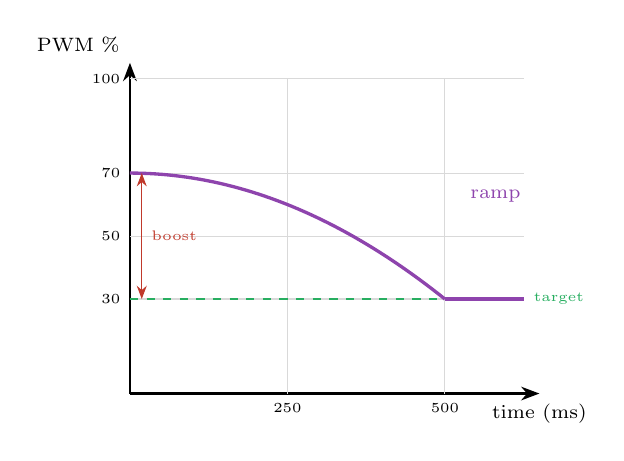
\begin{tikzpicture}
        \draw[-{Stealth}, thick] (0,0) -- (5.2,0)
          node[below, font=\scriptsize]{time (ms)};
        \draw[-{Stealth}, thick] (0,0) -- (0,4.2)
          node[above left, font=\scriptsize]{PWM \%};

        % Grid
        \foreach \y/\l in {1.2/30, 2.0/50, 2.8/70, 4.0/100} {
          \draw[gray!30] (0,\y) -- (5,\y);
          \node[left, font=\tiny] at (0,\y) {\l};
        }
        \foreach \x/\l in {2/250, 4/500} {
          \draw[gray!30] (\x,0) -- (\x,4);
          \node[below, font=\tiny] at (\x,0) {\l};
        }

        % Target speed = 30
        \draw[thick, dashed, sw] (0,1.2) -- (5,1.2)
          node[right, font=\tiny]{target};

        % Ramp curve (boost=70 decaying quadratically to 30)
        \draw[very thick, ctrl, domain=0:4, samples=50]
          plot (\x, {1.2 + 1.6*(1 - (\x/4)^2)});

        % After ramp
        \draw[very thick, ctrl] (4,1.2) -- (5,1.2);

        % Annotations
        \draw[{Stealth}-{Stealth}, thin, danger]
          (0.15,1.2) -- (0.15,2.8)
          node[midway, right, font=\tiny]{boost};

        \node[font=\scriptsize, text=ctrl, anchor=west] at (4.2,2.5)
          {ramp};
      \end{tikzpicture}
      }
    \end{column}
  \end{columns}
\end{frame}
\note{
Explain why the start ramp is needed: small DC motors may not move reliably at low PWM because of static friction. The algorithm briefly applies a higher boost and then smoothly decays to the requested speed. This makes starts more reliable without keeping the motor overpowered.
}

% ============================================================
\section{Wireless Communication}
% ============================================================

\begin{frame}{Wi-Fi Access Point \& REST API}

  \begin{columns}[T]
    \begin{column}{0.48\textwidth}
      The robot creates its own \textbf{Wi-Fi hotspot};
      the browser connects directly.

      \medskip
      {\small
      \begin{tabular}{@{}ll@{}}
        \toprule
        Setting & Value \\
        \midrule
        SSID     & \texttt{CodeCell-C6-Drive} \\
        Password & \texttt{12345678} \\
        IP       & \texttt{192.168.4.1} \\
        Protocol & HTTP (port 80) \\
        \bottomrule
      \end{tabular}
      }

      \bigskip
      \smallskip
      {\small REST commands use HTTP \texttt{GET} requests and JSON responses.}
    \end{column}

    \begin{column}{0.50\textwidth}
      \textbf{API Endpoints}

      \smallskip
      {\small
      \begin{tabular}{@{}lp{3.9cm}@{}}
        \toprule
        Endpoint & Purpose \\
        \midrule
        \texttt{/move}        & Joystick speed command\\[3pt]
        \texttt{/target}      & Distance + angle command\\[3pt]
        \texttt{/status}      & Battery, heading, motor state\\[3pt]
        \texttt{/estop}       & Emergency stop\\[3pt]
        \texttt{/clear\_estop} & Clear e-stop \\
        \bottomrule
      \end{tabular}
      }
    \end{column}
  \end{columns}
\end{frame}
\note{
Describe the communication setup. The robot creates its own Wi-Fi access point, so no external router is required. The browser sends simple HTTP GET requests to control movement, request status, and trigger or clear the emergency stop.
}

% ============================================================

\begin{frame}{Communication Flow}

  \centering
  \resizebox{!}{0.74\textheight}{%
  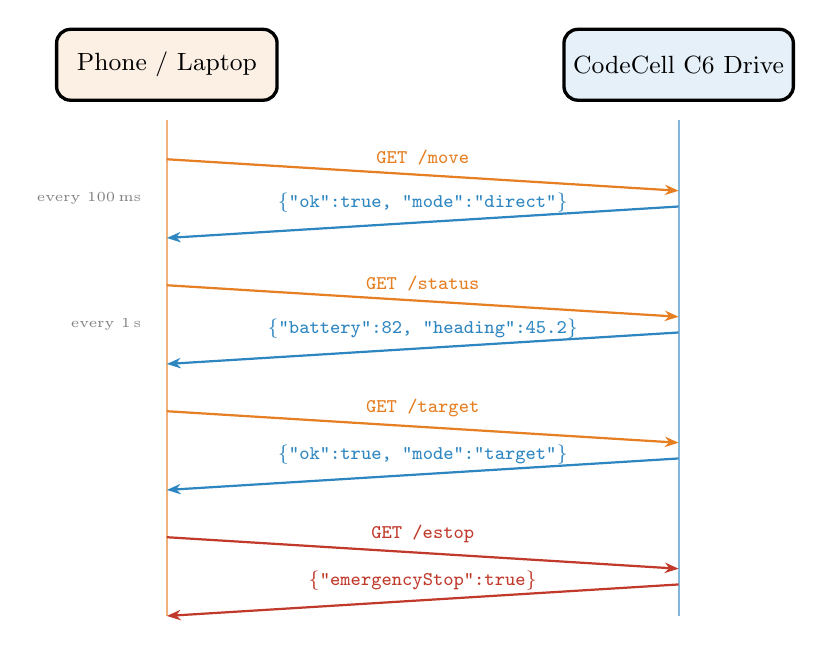
\begin{tikzpicture}[
      every node/.style={font=\small},
      entity/.style={draw, very thick, rounded corners=5pt,
                     minimum width=2.8cm, minimum height=0.9cm,
                     align=center},
      arr/.style={-{Stealth[length=5pt]}, thick},
      msg/.style={font=\scriptsize, midway}
    ]

    % Entities
    \node[entity, fill=comm!12] (phone) at (0,0)  {Phone / Laptop};
    \node[entity, fill=hw!12]   (robot) at (6.5,0)  {CodeCell C6 Drive};

    % Timeline
    \draw[thick, comm!60] (0,-0.7) -- (0,-7);
    \draw[thick, hw!60]   (6.5,-0.7) -- (6.5,-7);

    % Messages
    \draw[arr, comm] (0,-1.2) -- node[above, msg]
      {\texttt{GET /move}} (6.5,-1.6);
    \draw[arr, hw]   (6.5,-1.8) -- node[above, msg]
      {\texttt{\{"ok":true, "mode":"direct"\}}} (0,-2.2);

    \draw[arr, comm] (0,-2.8) -- node[above, msg]
      {\texttt{GET /status}} (6.5,-3.2);
    \draw[arr, hw]   (6.5,-3.4) -- node[above, msg]
      {\texttt{\{"battery":82, "heading":45.2\}}} (0,-3.8);

    \draw[arr, comm] (0,-4.4) -- node[above, msg]
      {\texttt{GET /target}} (6.5,-4.8);
    \draw[arr, hw]   (6.5,-5.0) -- node[above, msg]
      {\texttt{\{"ok":true, "mode":"target"\}}} (0,-5.4);

    \draw[arr, danger] (0,-6.0) -- node[above, msg]
      {\texttt{GET /estop}} (6.5,-6.4);
    \draw[arr, danger] (6.5,-6.6) -- node[above, msg, text=danger]
      {\texttt{\{"emergencyStop":true\}}} (0,-7.0);

    % Timing annotations
    \node[font=\tiny, text=gray, anchor=east] at (-0.2,-1.7) {every 100\,ms};
    \node[font=\tiny, text=gray, anchor=east] at (-0.2,-3.3) {every 1\,s};
  \end{tikzpicture}
  }
\end{frame}
\note{
Use this slide to explain the message sequence. The browser sends movement commands frequently, status is polled less often, target commands start autonomous motion, and emergency stop has a dedicated endpoint. Emphasize that the API is simple enough to test from any browser.
}

% ============================================================
\section{Control Application}
% ============================================================

\begin{frame}{Web-Based Control Interface}

  \begin{columns}[T]
    \begin{column}{0.47\textwidth}
      \textbf{Single-page HTML/JS app}
      \begin{itemize}
        \item Runs in any modern browser
        \item Touch-friendly virtual joystick
        \item Mouse and touch pointer events
      \end{itemize}

      \bigskip
      \textbf{Features}
      \begin{itemize}
        \item Joystick sends \texttt{/move} at 10\,Hz
        \item Target panel: distance, angle, IMU toggle
        \item Emergency stop / clear buttons
        \item Live status refreshed every second
      \end{itemize}
    \end{column}

    \begin{column}{0.50\textwidth}
      \centering
      \begin{tikzpicture}[
          scale=0.82,
          transform shape,
          every node/.style={font=\small},
          card/.style={draw, thick, rounded corners=5pt,
                       minimum width=4.8cm,
                       align=center, inner sep=6pt}
        ]

        \node[card, fill=comm!8] (conn) at (0,3.5)
          {\textbf{Connection}\\[-1pt]
           {\scriptsize IP: 192.168.4.1 \quad [Connect]}};

        \node[card, fill=ctrl!8] (joy) at (0,1.8)
          {\textbf{Joystick}\\[-1pt]
           {\scriptsize\begin{tikzpicture}[scale=0.35]
             \draw[thick, gray] (0,0) circle(1.2);
             \fill[ctrl!60] (0.3,-0.4) circle(0.4);
           \end{tikzpicture}}\\[-4pt]
           {\scriptsize Move: 45 \quad Rotation: -20}};

        \node[card, fill=sw!8] (tgt) at (0,0)
          {\textbf{Target Control}\\[-1pt]
           {\scriptsize Dist: 1.0\,m \quad Angle: 90$^\circ$ \quad IMU: off}};

        \node[card, fill=danger!8] (estop) at (0,-1.2)
          {\textbf{Emergency}\\[-1pt]
           {\scriptsize\fcolorbox{danger}{danger!30}{%
             \color{white}\bfseries STOP}
            \quad
            \fcolorbox{comm}{comm!30}{Clear}}};

        \node[card, fill=gray!8] (stat) at (0,-2.6)
          {\textbf{Status} (JSON)\\[-1pt]
           {\scriptsize battery, heading, motors, PID}};
      \end{tikzpicture}
    \end{column}
  \end{columns}
\end{frame}
\note{
Explain that the control application is a single-page web interface. It works on a phone or laptop and supports both mouse and touch input. Mention the main controls: connection, joystick, target command panel, emergency stop, and live status.
}

% ============================================================
\section{Safety \& Robustness}
% ============================================================

\begin{frame}{Safety Mechanisms}

  \begin{columns}[T]
    \begin{column}{0.48\textwidth}
      \textbf{\color{danger}Emergency Stop}
      \begin{itemize}
        \item One-click E-Stop via \texttt{/estop}
        \item All tasks check one shared flag
        \item Cleared only by explicit \texttt{/clear\_estop}
      \end{itemize}

      \bigskip
      \textbf{\color{comm}Command Timeout}
      \begin{itemize}
        \item Every command is timestamped
        \item No update within \textbf{300\,ms} $\rightarrow$ stop
        \item Handles Wi-Fi or browser failure
      \end{itemize}
    \end{column}

    \begin{column}{0.48\textwidth}
      \textbf{\color{ctrl}Thread Safety}
      \begin{itemize}
        \item Three FreeRTOS mutexes guard shared buffers
        \item No direct cross-task memory access
        \item Sequence counter detects new commands
      \end{itemize}

      \bigskip
      \textbf{\color{sw}Auto-Centre Joystick}
      \begin{itemize}
        \item On \texttt{pointerup}, joystick snaps to (0,\,0)
        \item Sends stop command immediately
        \item Prevents unintended continued motion
      \end{itemize}
    \end{column}
  \end{columns}
\end{frame}
\note{
Present safety as a core part of the design. Emergency stop overrides normal motion, command timeout stops the robot if communication is lost, mutexes protect shared state, and joystick auto-centering prevents the robot from continuing to move after input is released.
}

% ============================================================
\section{Summary \& Future Work}
% ============================================================

\begin{frame}{Summary}

  \begin{center}
  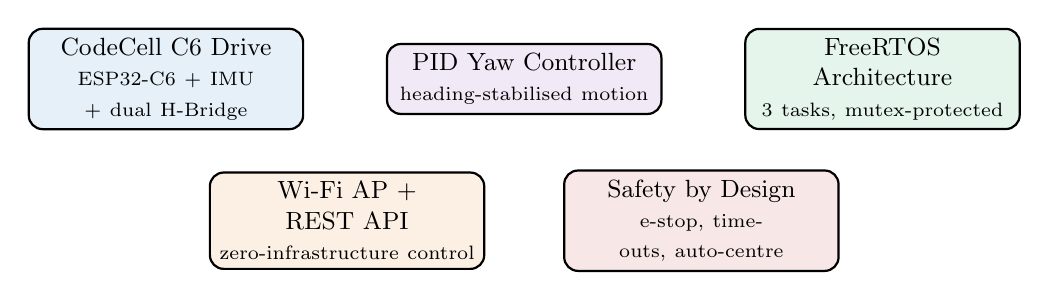
\begin{tikzpicture}[
      every node/.style={font=\small},
      summarybox/.style={draw, thick, rounded corners=5pt,
                   minimum width=3.45cm, minimum height=0.85cm,
                   text width=3.25cm, align=center}
    ]

    \node[summarybox, fill=hw!12]   (a) at (-4.55, 0.9) {CodeCell C6 Drive\\{\scriptsize ESP32-C6 + IMU + dual H-Bridge}};
    \node[summarybox, fill=ctrl!12] (b) at ( 0.0, 0.9) {PID Yaw Controller\\{\scriptsize heading-stabilised motion}};
    \node[summarybox, fill=sw!12]   (c) at ( 4.55, 0.9) {FreeRTOS Architecture\\{\scriptsize 3 tasks, mutex-protected}};
    \node[summarybox, fill=comm!12] (d) at (-2.25,-0.9) {Wi-Fi AP + REST API\\{\scriptsize zero-infrastructure control}};
    \node[summarybox, fill=danger!12](e) at ( 2.25,-0.9) {Safety by Design\\{\scriptsize e-stop, timeouts, auto-centre}};

  \end{tikzpicture}
  \end{center}

  \bigskip
  {\small
    A self-contained differential-drive robot built from one compact board,
    controlled from a browser, with real-time heading stabilisation from the
    onboard 9-axis IMU.
  }
\end{frame}
\note{
Summarize the project as a self-contained differential-drive robot built from a compact board with integrated wireless control, motor driving, and IMU feedback. Reinforce the main technical achievements: FreeRTOS architecture, PID heading control, browser control, and safety mechanisms.
}

% ============================================================

\begin{frame}{Future Work}

  \begin{itemize}
    \item \textbf{Obstacle avoidance} – reactive stop / turn behaviours

    \medskip
    \item \textbf{Odometry improvements} – wheel encoders or visual odometry

    \medskip
    \item \textbf{Multi-waypoint navigation} – sequence of target commands

    \medskip
    \item \textbf{BLE / Zigbee control} – lower-power communication options

    \medskip
    \item \textbf{Smartphone app} – richer UI and persistent settings
  \end{itemize}

\end{frame}
\note{
Mention practical extensions. Obstacle avoidance could use the proximity sensor, odometry could improve distance estimation, multi-waypoint navigation would make target mode more useful, and BLE/Zigbee or a smartphone app could improve the user experience.
}

% ============================================================

\begin{frame}[plain]
  \centering
  \vfill
  {\Huge\bfseries Thank you}

  \bigskip
  {\Large Questions?}

  \vfill

  {\small
    Source code \& 3D models available in the project repository
  }
\end{frame}
\note{
Close by inviting questions. Be ready to answer about PID tuning, communication reliability, mechanical design choices, and how the robot estimates distance in target mode.
}

\end{document}
